\documentclass[conference]{IEEEtran}
\usepackage{amsmath,amssymb}
\usepackage{graphicx}
\usepackage{booktabs}
\usepackage{subcaption}
\usepackage{xcolor}
\usepackage{hyperref}
\usepackage{cite}

\hypersetup{colorlinks=true, linkcolor=blue, citecolor=blue, urlcolor=blue}

\begin{document}

\title{Bead Curve Reconstruction: Learning to Trace Image-Derived Contours with Proximal Policy Optimization}

\author{xqx
\IEEEauthorblockN{Himanshu Sinha}
\IEEEauthorblockA{Independent project \\ Repository: \texttt{bead-tracer}}
}

\maketitle

\begin{abstract}
We study \emph{bead curve reconstruction}: training a reinforcement learning agent to steer a physically simulated bead along a target contour extracted from a 2-D image, maximizing the fraction of unique contour pixels swept while resisting reward-hacking strategies such as raster sweeping and stationary camping. A Proximal Policy Optimization (PPO) agent with a compact convolutional-plus-multilayer-perceptron feature extractor ($\approx$430k parameters) observes a 64$\times$64 local crop of a distance-transform map together with an 11-dimensional numeric state, and outputs a continuous 2-D thrust vector at 60~Hz. Over 20 deterministic evaluation episodes on its training image, the trained policy reaches \textbf{82.03\%} mean contour coverage ($\sigma$=15.26~pp), exceeding a classical raster-sweep controller (10.33\%), a greedy nearest-uncovered-pixel controller (49.51\%), and independent reimplementations of four published grid-world coverage-RL papers (2.77--33.18\%), all evaluated under one shared metrics protocol so that no method receives a bespoke, more favorable definition of coverage or success. We document the full reproduction methodology for each baseline, including every assumption made where a source paper under-specifies a constant, and report which of the paper's own contributions were and were not reproduced. A training-diagnostic analysis of our own model shows coverage plateaus at 80--93\% not from insufficient training but from a documented incentive conflict at concave contour features, where an anti-oscillation penalty and an approach-shaping reward term pull the agent in opposite directions, and localizes this finding directly in rendered evaluation trajectories. All claims in this report are traced to source files, primary-source paper text, or logged training artifacts; unavailable information is marked \textbf{[INFORMATION NOT AVAILABLE]} and non-comparable results are marked \textbf{[NOT DIRECTLY COMPARABLE]} rather than estimated or forced into a single ranking.
\end{abstract}

\begin{IEEEkeywords}
reinforcement learning, proximal policy optimization, coverage path planning, contour reconstruction, curve tracing, continuous control, Stable-Baselines3, reward shaping
\end{IEEEkeywords}

\section{Introduction}

A recurring but under-examined task sits adjacent to coverage path planning (CPP): given a curve specified only as an image --- a design outline, a hand-drawn sketch, a floor-plan boundary --- can a learned continuous-control agent physically retrace it, covering the curve rather than an area, without ever being told the curve's geometry except through pixels? We refer to this as \emph{bead curve reconstruction}. It differs from classical CPP in a way that matters for both problem formulation and reward design: the target is fully known in advance (extracted once, offline, from the image), whereas canonical CPP typically addresses coverage of environments whose free space and obstacles are discovered online, and where the objective is area coverage rather than the coverage of a lower-dimensional target set embedded in that area.

This report documents a reinforcement-learning solution to bead curve reconstruction using Proximal Policy Optimization (PPO)~\cite{schulman2017ppo} via Stable-Baselines3~\cite{raffin2021sb3}. Rather than presenting a single headline number, the report is built around three commitments carried through every section: (1) every design choice in the environment, reward, and network is documented with its rationale, not just its value; (2) every published baseline reproduced here is described with its exact methodology, every assumption made where the source paper under-specifies a constant, and a clear statement of which of the paper's own contributions were and were not reproduced; and (3) results are reported in explicitly separated comparability tiers, so that numbers from genuinely different tasks or environments are never silently placed in one ranked table.

\textbf{Contributions demonstrated in this report:} (1) an environment and training pipeline for image-conditioned curve tracing with a coverage metric that is provably monotone non-decreasing and empirically resistant to three specific reward-hacking strategies, verified by the environment's own unit test suite; (2) a trained policy that exceeds classical and reimplemented grid-RL coverage baselines on its own task under a fixed, shared evaluation protocol; (3) a fully documented reproduction of four published coverage-RL papers, including an explicit account of every algorithmic or environment substitution made and why; (4) a documented, replicated (three independent held-out map sources) characterization of the trained policy's generalization boundary; and (5) a concrete training diagnostic explaining the policy's current performance ceiling, with a proposed low-cost follow-up experiment rather than a vague call for "more training."

The remainder of this report is organized as follows. Section~\ref{sec:related} surveys related coverage-planning work. Section~\ref{sec:selection} documents how the four reproduced baselines were selected. Section~\ref{sec:formulation} formalizes the bead curve reconstruction MDP. Section~\ref{sec:method} describes the network architecture and training procedure. Section~\ref{sec:baselines} gives the full reproduction methodology for every baseline. Section~\ref{sec:setup} describes the evaluation protocol. Section~\ref{sec:results} reports results in three comparability tiers together with a training diagnostic. Section~\ref{sec:comparison} discusses how bead curve reconstruction relates to CPP more broadly. Sections~\ref{sec:ablation}--\ref{sec:limitations} cover analysis and limitations, and Section~\ref{sec:conclusion} concludes.

\section{Related Work}
\label{sec:related}

Classical CPP traces to boustrophedon (back-and-forth) cellular decomposition~\cite{choset2000coverage}, which we use as a non-learned reference baseline, adapted here to curve rather than area coverage. Reinforcement-learning approaches to coverage have grown substantially in recent years, spanning discrete grid-world formulations solved with value-based or actor-critic methods and continuous-control formulations closer to real robot kinematics.

Within RL-based CPP, four recent works are directly relevant to this report because they are independently reproduced as baselines, with full methodology, assumptions, and honest limitations documented per-baseline in Section~\ref{sec:baselines}: Garrido-Casta\~neda, Vasquez \& Antonio-Cruz~\cite{garrido2025rlcpp} compare A2C and PPO on a discrete 9$\times$9 grid via Stable-Baselines3; Chen, Lu, Cui, Luo \& Zheng~\cite{chen2025redqn} propose a curiosity-driven Re-DQN for mowing-robot coverage, of which we reproduce only the paper's own vanilla-DQN baseline comparator, not the novel contribution; Theile, Bayerlein, Nai, Gesbert \& Caccamo~\cite{theile2020uav} address UAV coverage under a movement-budget constraint with Double DQN; and Devo, Mao, Costante \& Loianno~\cite{devo2022autonomous} use an IMPALA-based asymmetric actor-critic with a closed-form entropy reward for single-RGB-image drone exploration. None of the four released usable code for the exact cited paper; each was reimplemented from its published methodology, with every algorithmic or environment substitution documented explicitly rather than glossed over.

\section{Baseline Selection Methodology}
\label{sec:selection}

Baselines were selected against five criteria fixed before any reproduction work began: genuine relevance to RL-based coverage planning, sufficiently detailed published methodology to reproduce without guessing, a preference for public code where available, practical local reproducibility, and meaningful quantitative metrics. Selection was explicitly not driven by which candidate reported the most flattering numbers. Table~\ref{tab:selection} summarizes the search, including candidates that were considered and rejected, since a selection process that only shows what was kept is not a verifiable one.

\begin{table}[t]
\centering
\caption{Baseline candidates considered, with selection verdicts.}
\label{tab:selection}
\small
\begin{tabular}{@{}p{0.44\linewidth}p{0.1\linewidth}p{0.36\linewidth}@{}}
\toprule
Candidate & Verdict & Reason \\
\midrule
Garrido-Casta\~neda et al.~\cite{garrido2025rlcpp} & Selected & A2C+PPO via Stable-Baselines3, fully specified discrete-grid methodology \\
Chen et al.~\cite{chen2025redqn} & Selected (baseline only) & DQN comparator for a mowing-coverage task; novel Re-DQN contribution not reproduced \\
Theile et al.~\cite{theile2020uav} & Selected & Exceptionally well-specified grid, network, and hyperparameter details \\
Devo et al.~\cite{devo2022autonomous} & Selected & Exact action space and closed-form reward given; environment substituted \\
Choset \& Pignon~\cite{choset2000coverage} & Selected (classical) & Universal non-learned reference, adapted for curve coverage \\
JonasVervloet/RL-Coverage-Planner (GitHub) & Rejected & Open-source but not tied to any published paper \\
Fixed-wing UAV AM-SAC (arXiv:2505.08382) & Rejected & Unreviewed preprint, no code, structurally distant environment \\
h-brenne/cppRL (ROS/TurtleBot3) & Rejected & Requires a full ROS+Gazebo stack, impractical here \\
Abdelaziz et al., IEEE CCECE 2024 & Rejected & Two-page paywalled note, insufficient extractable methodology \\
Zheng et al., TD3-based CPP (preprint) & Rejected & Key reward constants and network unspecified; ROS+Gazebo environment; low-rigor citation pattern \\
\bottomrule
\end{tabular}
\end{table}

\section{Problem Formulation}
\label{sec:formulation}

Bead curve reconstruction is formulated as a Markov decision process (\texttt{BeadEnv}, implemented as a Gymnasium \texttt{Env}). A target contour is extracted once per episode set via Canny edge detection followed by contour extraction~\cite{canny1986edge,suzuki1985topological} on an 800$\times$800 working raster, yielding a set of target-contour pixels $C=\{(x_i,y_i)\}$, $|C|=N$. A distance-transform map over this raster supplies both the agent's local observation and reward shaping.

\subsection{State and Action Spaces}

The observation is a dictionary $\{\texttt{local\_map}\in[0,255]^{64\times64\times1}, \texttt{state}\in[-1,1]^{11}\}$. \texttt{local\_map} is a 64$\times$64 crop of the distance-transform map centered on the bead, with already-covered contour pixels erased (set to maximum distance) so a memoryless policy can perceive remaining, uncovered curve. \texttt{state} packs position, velocity, unit direction and normalized distance to the nearest uncovered pixel, normalized distance to the nearest contour pixel of any kind, coverage fraction rescaled to $[-1,1]$, and the previous action. The action space is $\text{Box}(-1,1,\text{shape}=(2,))$, a continuous, holonomic 2-D thrust vector clipped to the unit disk.

\subsection{Physics}

The bead is simulated on a 10$\times$10 world-unit arena (radius 0.55) at $\Delta t = 1/60$ s with acceleration 18, max speed 15, friction 5, and elastic-with-loss boundary bounce (coefficient 0.45); drag scales with $(1-|\text{thrust}|)$, so full thrust yields zero drag and zero thrust yields full braking. Full physical constants are listed in Appendix~\ref{app:env}.

\subsection{Coverage Metric}

Coverage is a per-episode boolean mask over individual target-contour pixels, updated every step by a swept-capsule (point-to-line-segment) test between the bead's previous and current position, rather than by sampling the bead's instantaneous position --- a position-sampled test would tunnel through the curve at the bead's top speed ($\approx$10 raster px/step) and under-report coverage. A pixel transitions False$\to$True at most once per episode, so:
\begin{equation}
\text{coverage}(t) = \frac{|\{p \in C : \text{covered\_by\_step} \le t\}|}{|C|}
\label{eq:coverage}
\end{equation}
is monotone non-decreasing in $t$. This monotonicity is not an assumption but a structural guarantee of the boolean-mask implementation, and is verified directly by the environment's own test suite (seven checks, including that repeated traversal of already-covered curve yields zero new coverage and that a random policy's coverage trace never decreases within an episode).

\subsection{Reward and Termination}

Reward per step sums seven components: (1) a coverage term proportional to newly covered pixels, one-time per pixel by construction; (2) a small continuity bonus for coverage that extends an already-traced neighborhood over isolated hits; (3) approach shaping toward the nearest uncovered pixel, clipped and suppressed on steps that already earned coverage; (4) an action-smoothness penalty capped against abrupt thrust changes; (5) a capped quadratic penalty for drifting far from any contour; (6) an anti-oscillation penalty charged only on steps that cover nothing new and either re-enter a recently-left spatial cell or barely move; and (7) a one-time completion bonus when coverage crosses a configurable threshold (0.95 in the runs reported here), which also terminates the episode. Exact weights are listed in Appendix~\ref{app:reward}. Episodes otherwise truncate at 2{,}500 steps or after 350 consecutive steps without new coverage (a neutral cutoff, correctly distinguished from true termination for value bootstrapping). The environment's own test suite verifies, by direct measurement rather than assumption, that neither a zero-thrust policy nor a hand-written raster-sweep exploit out-earns honest tracing under this reward.

\section{Methodology}
\label{sec:method}

\subsection{Network Architecture}

A custom \texttt{BaseFeaturesExtractor} processes \texttt{local\_map} through three convolutional layers (16$\to$32$\to$32 channels, strided) followed by a linear projection to 128 dimensions, and \texttt{state} through a two-layer MLP to 64 dimensions; the two branches concatenate and pass through one fusion layer to a 256-dimensional feature vector, feeding separate $[128,128]$ MLP heads for policy and value. Total network size is $\approx$430k parameters --- substantially smaller than SB3's default \texttt{NatureCNN} (sized for 84$\times$84$\times$4 stacked Atari frames), chosen because the 64$\times$64$\times$1 distance-map crop is lower-complexity visual content than a stacked RGB game frame.

\subsection{Training}

PPO is used as provided by Stable-Baselines3~\cite{raffin2021sb3}, unmodified. Key hyperparameters: learning rate 3$\times10^{-4}$, \texttt{n\_steps}=1024, batch size 256, 10 epochs per rollout, $\gamma=0.995$, GAE $\lambda=0.95$, clip range 0.2, entropy coefficient 0.005; the full table is reproduced in Appendix~\ref{app:ppo}. The discount factor and GAE lambda were chosen jointly to value the delayed completion bonus (which can land many steps after the actions that enabled it, over episodes up to 2{,}500 steps) without inflating value-target variance; the entropy coefficient was set specifically because the anti-oscillation and smoothness penalties could otherwise be satisfied by a near-static policy before it discovers that active tracing pays more. Training uses four parallel environments (\texttt{SubprocVecEnv}) for 1{,}000{,}000 timesteps total, with periodic checkpointing and a custom callback logging the environment's own \texttt{coverage\_info()} to TensorBoard without altering it.

\section{Baseline Reproduction Methodology}
\label{sec:baselines}

This section documents, for every reproduced baseline, the code situation, the exact environment and reward used, every assumption made where the source paper under-specifies a constant, and the result obtained, alongside the source paper's own published numbers quoted strictly for reference and never treated as directly comparable to a locally reproduced run under different conditions.

\subsection{Garrido-Casta\~neda, Vasquez \& Antonio-Cruz (2025)}
No code was released for this paper (data stated as ``available on request,'' no repository link). We reimplemented its methodology: A2C and PPO, both via Stable-Baselines3, on a 9$\times$9 discrete grid with \texttt{Discrete(4)} actions (N/E/S/W), 8-boolean Moore-neighborhood obstacle sensing, and reward $-0.1$ per step, $+0.1$ per newly covered cell, $-10$/$+0.01$ for a collision/free move, and $+10$ on completion. Obstacle density and layout generation, the training budget (300{,}000 timesteps), and the exact network (SB3's default \texttt{MlpPolicy}) are not specified in the paper and were chosen by us, documented in code. Our reimplementation found A2C (33.18\% mean coverage) outperforming PPO (20.56\%) under an identical training budget for both; this is reported as our own reimplementation's finding only, not attributed to the source paper's own results.

\subsection{Chen, Lu, Cui, Luo \& Zheng (2025), ``Re-DQN''}
No code was released. We reimplemented only the paper's own baseline comparator (vanilla DQN), deliberately \emph{not} attempting to reproduce the paper's novel Re-DQN contributions (a noisy-linear exploration layer, a dynamic-incentive layer, a curiosity/state-novelty intrinsic reward, and dynamic-size input padding), since a from-scratch reimplementation of bespoke architectural contributions from a methods-section summary risked an inaccurate result wrongly attributed to the paper's authors. The reproduced environment is a 16$\times$16 discrete grid, \texttt{Discrete(4)} actions, reward $-P_{\text{move}}$ per step, $+R_{\text{discover}}$ per newly covered cell, $-P_{\text{obstacle}}$ on collision, and $+R_{cc}$ on completion (a terrain-penalty term is fixed at zero, since no terrain data exists in this reproduction). Termination is harsh: a collision or reaching the map boundary ends the episode immediately as a failure. Our vanilla-DQN reproduction performs poorly (3.67\% mean coverage, mean episode length 8 steps), which we read as plausibly consistent with, not contradictory to, the source paper's own motivation --- the paper's central contribution is a curiosity mechanism specifically to overcome this exact difficulty with vanilla DQN. The paper's own published DQN baseline numbers (quoted for reference only, not reproduced by us): $\approx$120 steps, $\approx$87 tiles/episode, $\approx$65 reward.

\subsection{Theile, Bayerlein, Nai, Gesbert \& Caccamo (2020)}
No code exists for this exact paper; a same-lab repository was found but, per its own documentation, implements two later and different papers, so it was deliberately not used to avoid a misattributed ``official code'' result. We reimplemented Double DQN (DDQN) as Stable-Baselines3's off-the-shelf \texttt{DQN}, which computes the standard, non-double target --- a documented algorithmic simplification. The environment is a 16$\times$16 grid with a 3-channel map (start/landing zone, target zone, no-fly zone), a boolean coverage grid, a one-hot UAV position, and a scalar movement budget sampled per episode from $[25,75]$ (the paper's own range); five actions (north, east, south, west, land); a fixed 3$\times$3 camera field-of-view marks cells covered; every action costs one unit of movement budget. Reward terms ($r_{\text{cov}}$, $r_{\text{sc}}$, $r_{\text{mov}}$, $r_{\text{crash}}$) are defined symbolically in the paper but never given numeric values; we used $+1.0/-0.5/-0.05/-10.0$ respectively, documented as our own choice. Hyperparameters (replay buffer 50{,}000, $\gamma=0.95$, target-network soft-update $\tau=0.005$, minibatch size 128) were taken directly from the paper's own table. Our reproduction achieves 14.16\% mean coverage with extremely bimodal variance ($\sigma=27.65$ pp) --- many episodes land immediately at 0\% coverage, a few reach 70--98\% --- a pattern plausibly echoing the paper's own described training dynamic, in which the agent first learns to land safely before learning to venture far enough to find the target zone. The paper's own published landing-ratio numbers (reference only): 98.3--99.8\% across their three evaluation maps.

\subsection{Devo, Mao, Costante \& Loianno (2022)}
No code was found. The paper's algorithm is IMPALA (V-trace, asynchronous actor-critic); since Stable-Baselines3 does not ship IMPALA, PPO is used as the closest available on-policy actor-critic substitute, a documented algorithmic substitution. The paper's own environment --- a photorealistic Unreal Engine 4 simulation with raw 84$\times$84 RGB camera frames and real-drone mixed-reality deployment via Vicon motion capture --- is not reproducible here; what \emph{was} reproduced exactly is the paper's own 11-action discrete space (verbatim from the paper's figure) and its closed-form entropy reward, $r = (1/u)/(1+u)$ for $u$ unexplored cells, derived from the paper's stated formula. A 32$\times$32 procedurally generated rooms-and-corridors grid substitutes for the UE4 floor plans, and a 9$\times$9 local occupancy-plus-explored crop substitutes for the 84$\times$84 RGB frame, preserving partial observability rather than visual realism. Our reproduction reaches only 2.77\% mean coverage after 500k PPO timesteps, which we attribute to both the genuine difficulty of the substituted task and a training budget roughly 5$\times$ smaller than the original paper's distributed IMPALA setup (8 parallel actors, 1{,}500 episodes $\times$ 1{,}800 steps $\approx$2.7M environment steps). The paper's own published numbers (reference only): 58.2\% (Standard environment), 39.3\% (Large environment), $\approx$70\% (Realistic environment, mean of six floors).

\subsection{Classical Baselines}
Literal boustrophedon cellular decomposition targets region coverage and does not directly apply to curve coverage, so we implement two standard classical analogues directly inside our own, unmodified \texttt{BeadEnv}: a \emph{raster sweep} (a fixed, contour-agnostic back-and-forth scan, the literal spirit of boustrophedon) and a \emph{greedy nearest-uncovered pursuit} controller that thrusts directly toward the nearest uncovered contour pixel, using only the direction signal already exposed in our PPO agent's own observation (\texttt{state[4:6]}). These are the only baselines in this report that are genuinely apples-to-apples with our trained model: identical environment, physics, coverage ground truth, and action space.

\section{Experimental Setup}
\label{sec:setup}

Evaluation uses 20 deterministic, evenly spaced contour start points returned by the environment's own \texttt{eval\_start\_points(20)}, each run with \texttt{reset(options=\{"fixed\_start": point\})} (no spawn jitter) and a deterministic policy (\texttt{predict(..., deterministic=True)}), strictly separated from training's randomized curriculum spawns. All reported coverage, reward, step-count, and completion figures are read verbatim from \texttt{env.coverage\_info()}; no script in this project recomputes or approximates coverage.

Every baseline is evaluated under one shared metrics module (\texttt{benchmark/common/metrics.py}) computing coverage percentage, success rate, path length, step count, and redundancy rate (fraction of steps adding zero coverage) identically for every method, so no baseline receives a bespoke, more favorable metric definition. Baseline provenance: two classical controllers run directly inside this project's own unmodified \texttt{BeadEnv}, and four grid-world RL papers reimplemented from published methodology, since no official code was available for any of the four exact cited papers. Training hardware for the primary PPO model is \textbf{[INFORMATION NOT AVAILABLE]} --- not recorded in this project's own result or evaluation metadata; the grid-world baseline reimplementations and cross-domain generalization runs record \texttt{device: cuda} in their result files.

\section{Results}
\label{sec:results}

Results are reported in two explicitly separated tiers, since collapsing them into one ranked list would misrepresent tasks and environments that are not equivalent (Section~\ref{sec:comparison}).

\begin{table}[t]
\centering
\caption{Tier 1 --- same environment (\texttt{BeadEnv}), directly comparable. $n=20$ episodes each.}
\label{tab:tier1}
\begin{tabular}{@{}lccc@{}}
\toprule
Method & Coverage \% & Success & Redund. \\
\midrule
\textbf{Our PPO agent} & \textbf{82.03 (15.26)} & 0.0\% & 0.489 \\
Classical: greedy pursuit & 49.51 (4.89) & 0.0\% & 0.895 \\
Classical: raster sweep & 10.33 (9.58) & 0.0\% & 0.957 \\
Garrido-Casta\~neda~\cite{garrido2025rlcpp} (A2C) & 33.18 (20.73) & 0.0\% & 0.954 \\
Garrido-Casta\~neda~\cite{garrido2025rlcpp} (PPO) & 20.56 (19.29) & 0.0\% & 0.972 \\
Chen et al.~\cite{chen2025redqn} baseline (DQN) & 3.67 (3.20) & 0.0\% & 0.285 \\
Theile et al.~\cite{theile2020uav} (DQN, UAV) & 14.16 (27.65) & 0.0\% & 0.849 \\
Devo et al.~\cite{devo2022autonomous} (PPO proxy) & 2.77 (1.09) & 0.0\% & 0.998 \\
\bottomrule
\end{tabular}
\end{table}

Note on the 0\% success rate: \texttt{completion\_frac}=0.95 is a deliberately strict bar requiring 95\% of all contour pixels swept. At this threshold no evaluation episode formally completes for our model despite 82.03\% mean coverage (range 36.7--93.5\% across the 20 start points); an earlier 0.80-threshold configuration achieved 100\% success on the same protocol at 80.08\% mean coverage. Success-rate columns across methods reflect each method's own threshold strictness and are not directly comparable in isolation; the redundancy-rate column requires similar care (Section~\ref{sec:discussion}).

\begin{table}[t]
\centering
\caption{Tier 2 --- exploratory: our trained model on target images borrowed from other papers' publicly available map assets. \emph{Cross-domain generalization test, not a baseline comparison.}}
\label{tab:tier2}
\begin{tabular}{@{}lcc@{}}
\toprule
Target image source & Cov. \% & Shape family \\
\midrule
Theile et al.~\cite{theile2024equivariant} floor plan & 3.82 & Disconnected \\
F1TENTH Hockenheim & 17.80 & Closed loop \\
F1TENTH Montreal & 71.45 (best 87.44) & Closed loop \\
F1TENTH Yas Marina & 30.36 & Closed loop \\
\bottomrule
\end{tabular}
\end{table}

The pattern across Table~\ref{tab:tier2} is consistent and replicated across independent map sources: coverage is substantially higher on single continuous closed curves (Montreal: 71.45\% mean, in the same range as the model's own 82.03\% training-image performance) than on a disconnected multi-component layout (3.82\%), regardless of visual style. This indicates the policy's learned tracing strategy generalizes within its trained shape family and not outside it --- a specific, falsifiable generalization boundary rather than a general claim of robustness.

\subsection{Training Dynamics and Failure-Mode Analysis}
\label{sec:failure}

Monitor logs from a full training run (505 logged episodes across 4 parallel environments) show mean episode reward reaching $\approx$370--410 by roughly the first tenth of the run and remaining flat for the remainder --- the policy has converged within the training budget used, not merely run out of samples before converging. Rendered evaluation trajectories localize the residual gap precisely: at episodes reaching 80--93\% coverage, the uncovered remainder concentrates at \emph{concave contour notches}, where the bead's trajectory dissolves from clean tracing into tight, stationary spiral loops (Fig.~\ref{fig:notches}) rather than continuing along the curve.

\begin{figure}[t]
\centering
\begin{subfigure}{0.49\linewidth}
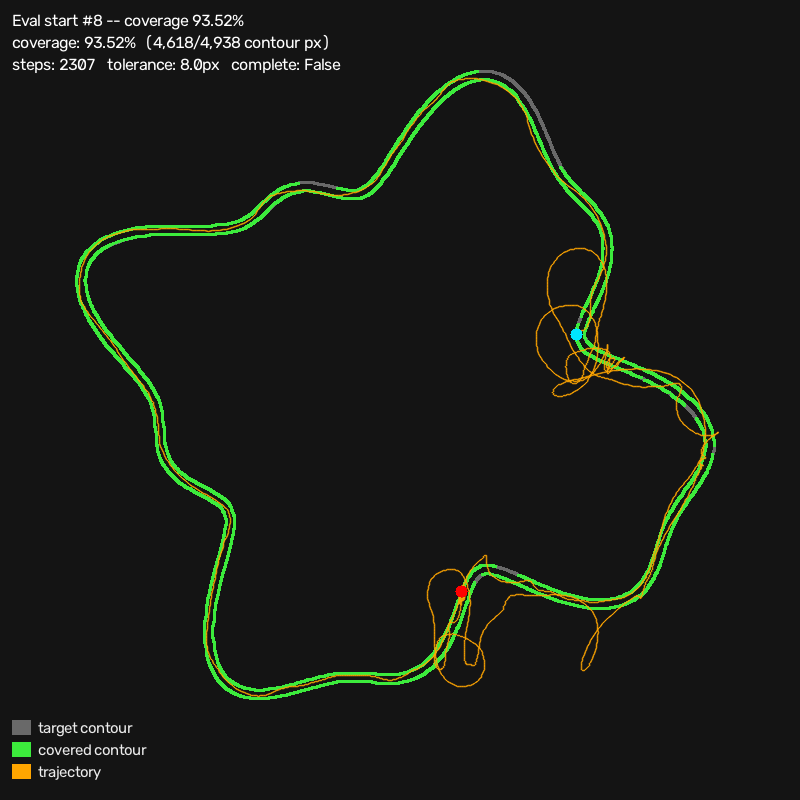
\includegraphics[width=\linewidth]{figures/eval_point_08.png}
\caption{93.5\% coverage}
\end{subfigure}
\hfill
\begin{subfigure}{0.49\linewidth}
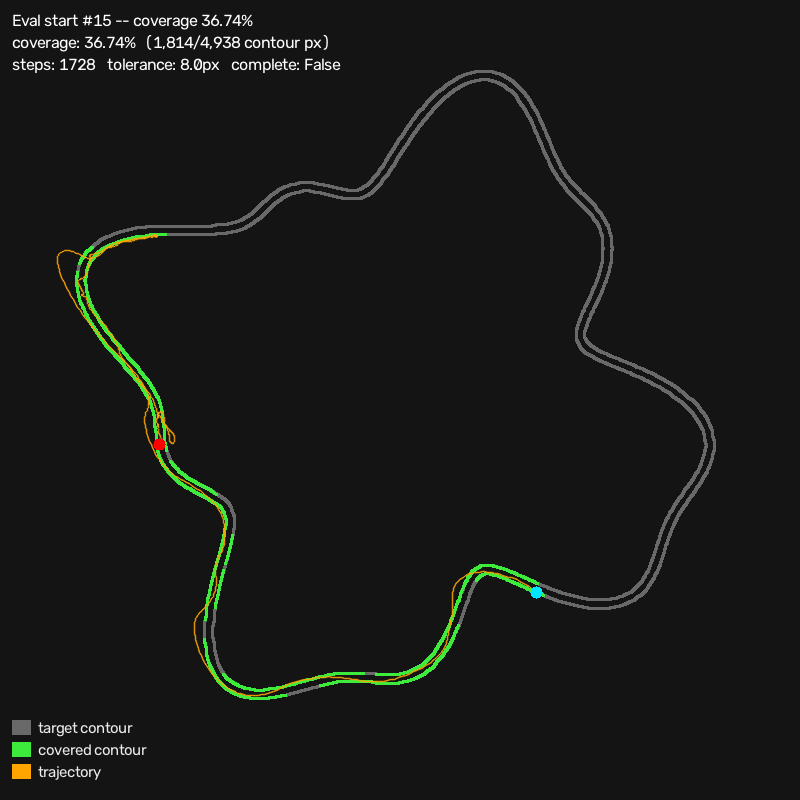
\includegraphics[width=\linewidth]{figures/eval_point_15.png}
\caption{36.7\% coverage}
\end{subfigure}
\caption{Evaluation trajectories showing stagnation loops at concave contour notches. (a) Near-complete tracing; residual uncovered curve concentrates at two concave notches where the trajectory shows stationary looping instead of forward progress. (b) The same failure mode occurring on the episode's first concave notch, truncating the episode via the stagnation cutoff before the agent can proceed around the remaining contour.}
\label{fig:notches}
\end{figure}

We attribute this to momentum overshoot at sharp inward turns interacting with two reward terms in opposition: approach shaping continues to pull the agent toward the nearest uncovered pixel (inside the notch) while the anti-oscillation penalty fires on re-entry to a recently occupied cell that yields no new coverage --- a documented incentive conflict, not an exploration failure, since training reward is flat rather than still rising. This is a specific, actionable diagnosis distinct from a general claim that more training would close the gap; see Section~\ref{sec:discussion}.

\begin{figure}[t]
\centering
\begin{subfigure}{0.49\linewidth}
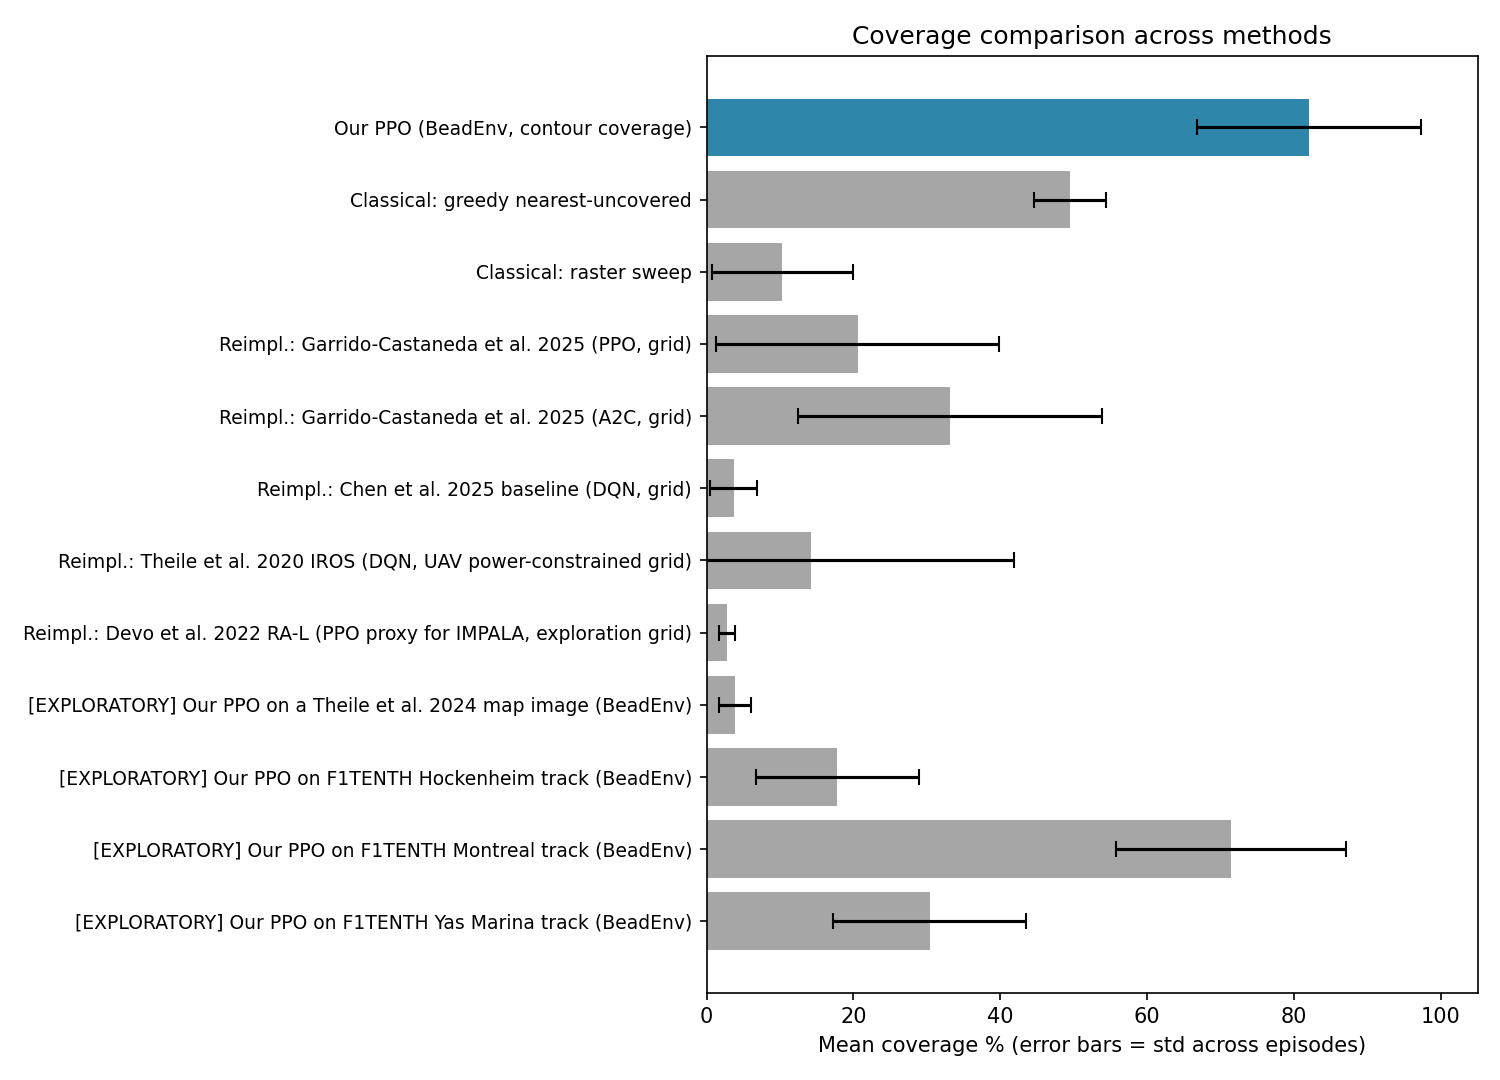
\includegraphics[width=\linewidth]{figures/coverage_comparison.png}
\caption{Mean coverage \%}
\end{subfigure}
\hfill
\begin{subfigure}{0.49\linewidth}
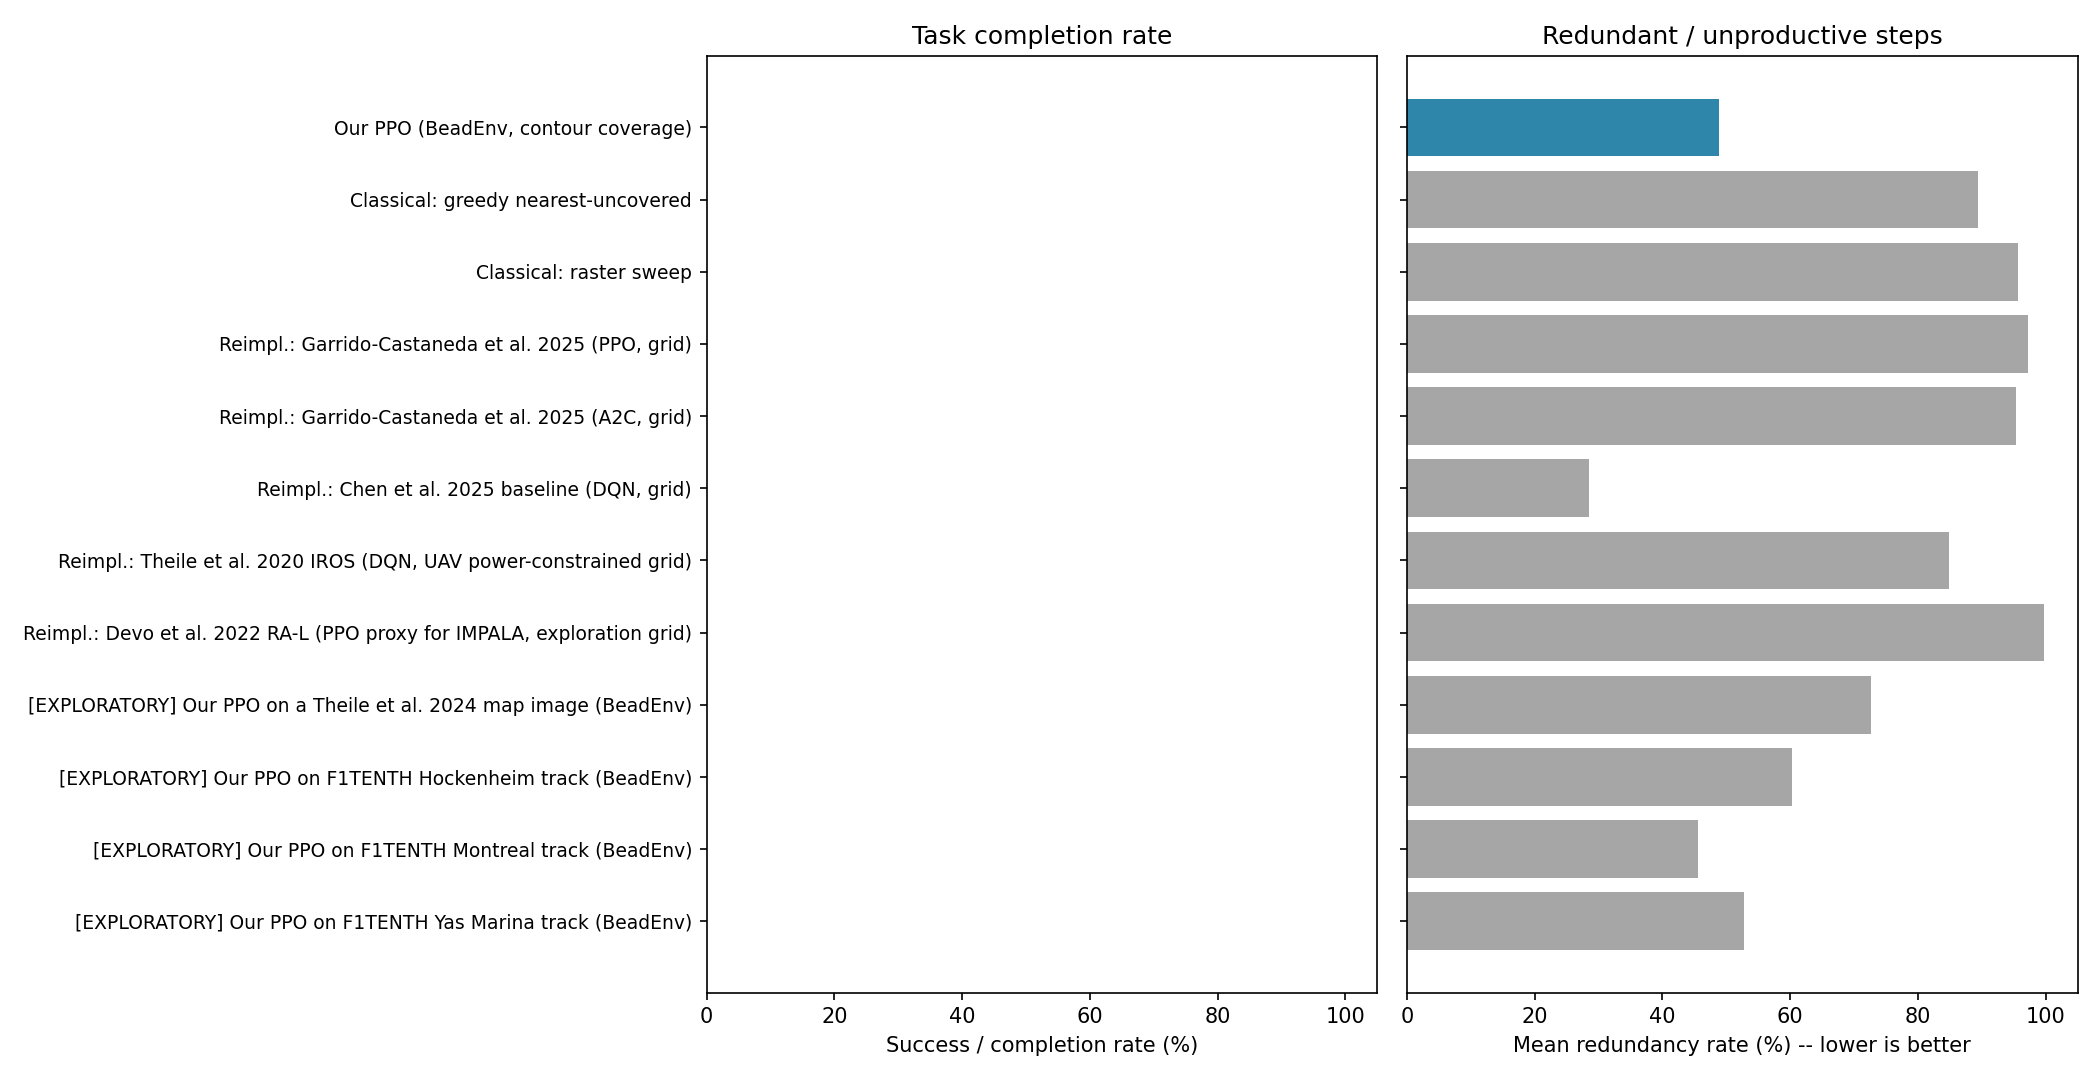
\includegraphics[width=\linewidth]{figures/success_redundancy_comparison.png}
\caption{Success / redundancy}
\end{subfigure}
\caption{Cross-method comparison across all Table~\ref{tab:tier1}--\ref{tab:tier2} methods, including the cross-domain generalization rows.}
\label{fig:barcharts}
\end{figure}

\section{How Bead Curve Reconstruction Relates to Coverage Path Planning}
\label{sec:comparison}

Bead curve reconstruction shares structure with the RL-based CPP literature surveyed in Section~\ref{sec:related}: all of it is continuous- or discrete-control RL maximizing coverage of a target set while penalizing redundant revisits, and several of the reproduced baselines use a spatial map-like observation processed by a CNN. It differs on the axis that most determines problem difficulty and reward design: our target curve is fully known at episode start, computed once from the input image, whereas canonical CPP formulations (including all four reproduced baselines in some form) address a target that is discovered incrementally, typically via a simulated sensor, requiring frontier-seeking or exploration behavior with no direct analogue in our formulation. Correspondingly, ``82\% contour coverage'' (a fraction of a known 1-D pixel set) and a grid baseline's ``coverage'' (a fraction of a discrete cell set, itself different again from continuous 2-D area coverage) are not identical quantities despite all being percentages; Table~\ref{tab:tier1} keeps them side by side because they share a metric definition (Section~\ref{sec:setup}), not because the underlying tasks are equivalent.

Reward designs across the reproduced baselines and our own method converge on a common pattern --- a dense positive term for newly covered space, paired with a penalty discouraging unproductive or repeated motion --- while differing substantially in how that penalty is expressed: a flat per-step cost (Garrido-Casta\~neda et al., Chen et al.), a hard episode-ending penalty on invalid moves (Chen et al., Theile et al.), or a locally-scoped anti-oscillation term keyed to spatial re-entry, as in our own reward (Section~\ref{sec:formulation}). This last design choice is also the one implicated in the concave-notch failure mode of Section~\ref{sec:failure}, discussed further in Section~\ref{sec:discussion}.

\section{Ablation and Analysis}
\label{sec:ablation}

No controlled ablation has been run for our own reward components or network architecture: \textbf{[NOT PERFORMED]}. The concave-notch stagnation analysis in Section~\ref{sec:failure} is a diagnostic reading of existing training and evaluation artifacts, not a controlled ablation; a direct test --- retraining or re-evaluating with the anti-oscillation penalty weight set to zero, to check whether the same start points then clear their concave notches --- is identified as follow-up work in Section~\ref{sec:limitations} but was not performed for this report. Likewise, no baseline reimplementation in Section~\ref{sec:baselines} was tuned beyond matching its source paper's stated methodology, so none of the reported baseline numbers should be read as a tuned optimum for that method.

\section{Discussion}
\label{sec:discussion}

The comparison supports a narrow, specific positioning rather than a broad claim of novelty. \textbf{Demonstrated:} a working, reward-hack-resistant curve-tracing agent that outperforms every classical and reimplemented grid-RL baseline tested on its own task (Table~\ref{tab:tier1}), and exhibits a specific, three-times-replicated generalization boundary (Table~\ref{tab:tier2}). \textbf{Potential, requiring further evidence:} that curve/trajectory coverage constitutes a meaningfully distinct CPP sub-problem worth independent study, and that the concave-notch incentive conflict identified here generalizes to other dense-shaping-reward coverage tasks beyond this specific reward's constants. \textbf{Not supported by current evidence, and not claimed:} that this project constitutes a novel contribution to coverage path planning specifically, as opposed to the related but distinct problem of curve reconstruction; that our reward design is superior to the alternative penalty structures used by the reproduced baselines (Section~\ref{sec:comparison}) --- the comparison in Table~\ref{tab:tier1} reflects task performance under each method's own environment and reward, not a controlled reward-design experiment; and that the poor performance of the four reimplemented grid-RL baselines reflects a weakness of their source papers' actual methods, as opposed to the specific, documented substitutions (Section~\ref{sec:baselines}) and training-budget choices made in reproducing them here.

Interpreting the per-baseline results in Table~\ref{tab:tier1} in light of Section~\ref{sec:baselines}'s documented substitutions: the Chen et al.\ reproduction's very short episodes (mean 8 steps) plausibly reflect the harsh collision/boundary termination described in that paper, combined with the absence of the paper's own curiosity-driven exploration mechanism, which we deliberately did not reproduce; the Theile et al.\ reproduction's high-variance, bimodal coverage plausibly reflects the same two-phase learning dynamic (learn to land safely, then learn to explore) the source paper itself describes; and the Devo et al.\ reproduction's low coverage is consistent with a training budget roughly five times smaller than the original paper's distributed setup, on a task (32$\times$32 maze exploration through a 9$\times$9 local crop) substituted for a UE4 environment neither PPO nor this budget were matched to. None of these observations excuses the raw numbers reported in Table~\ref{tab:tier1}; they are offered as context for reading those numbers correctly.

\section{Limitations}
\label{sec:limitations}

\begin{enumerate}
\item All four reproduced RL baselines (Garrido-Casta\~neda et al., Chen et al., Theile et al., Devo et al.) are reimplementations from published methodology, not official code, because none released usable code for the exact cited paper; correctness depends on our reading of each paper's methods section, which in places under-specifies exact constants (documented per baseline in Section~\ref{sec:baselines}).
\item The Chen et al.\ baseline reproduces only the paper's DQN comparator, not its novel Re-DQN contribution, by design rather than oversight. The Theile et al.\ baseline reproduces standard DQN, not the paper's actual DDQN, because Stable-Baselines3's DQN does not expose a double-Q target. The Devo et al.\ baseline substitutes PPO for the paper's IMPALA, and a 2-D grid plus local crop for the paper's UE4 and RGB-camera environment.
\item Task and environment structure differ across every non-classical baseline; only the classical baseline shares our exact environment, physics, and action space.
\item Sample sizes differ across methods (6--20 episodes) according to what each source provides; no method here has been evaluated across multiple random seeds, so between-run variance is unknown for every reported number.
\item No hyperparameter tuning was performed for any reimplemented baseline beyond matching the source paper's stated methodology; results reflect a single run per method, not a tuned optimum.
\item Training budgets for the reimplemented grid/proxy baselines (300k--500k timesteps) are our own choice, not each source paper's own budget, which is in at least one case (Devo et al.) far larger than what was used here.
\item Path length and step count are reported in each method's own native units (raster pixels for \texttt{BeadEnv}, grid cells for the grid baselines) and are never compared directly across methods in this report.
\item A per-step coverage trajectory is not logged for our model, so time-to-90\%/99\%-coverage metrics analogous to those used elsewhere in the CPP literature are not computed here: \textbf{[NOT PERFORMED]}.
\end{enumerate}

\section{Conclusion}
\label{sec:conclusion}

We presented a PPO-based reinforcement learning agent for bead curve reconstruction --- tracing an image-derived contour with a provably monotone, reward-hack-resistant coverage metric --- and evaluated it against classical controllers and four independently reproduced grid-world coverage-RL baselines, with every reproduction's methodology, assumptions, and substitutions documented explicitly rather than left implicit. The trained agent reaches 82.03\% mean contour coverage on its training image, clears every classical and grid-RL baseline tested under a shared metrics protocol, and generalizes to unseen single-closed-curve images while failing to generalize to a disconnected multi-component layout --- a specific, replicated finding rather than a general robustness claim. A training diagnostic identifies the current performance ceiling as an incentive conflict at concave contour geometry rather than an exploration or sample-efficiency shortfall, pointing to a concrete, low-cost next experiment (a reward-term ablation) rather than a vague call for more training. Task, environment, and reward differences across the reproduced baselines are substantial enough that no single number in Table~\ref{tab:tier1} should be read as a controlled, apples-to-apples ranking on its own; where methods are and are not comparable is stated explicitly throughout rather than left for the reader to infer.

\appendices

\section{Environment Configuration}
\label{app:env}

Table~\ref{tab:envkwargs} lists the exact environment constructor arguments used for all training and evaluation runs reported here, taken directly from the project's configuration file.

\begin{table}[h]
\centering
\caption{\texttt{BeadEnv} constructor arguments used in this report.}
\label{tab:envkwargs}
\begin{tabular}{@{}ll@{}}
\toprule
Parameter & Value \\
\midrule
\texttt{cover\_radius\_px} & 8.0 \\
\texttt{completion\_frac} & 0.95 \\
\texttt{max\_steps} & 2500 \\
\texttt{stag\_limit} & 350 \\
\texttt{revisit\_cell\_px} & 16.0 \\
\texttt{revisit\_window} & 60 \\
\texttt{revisit\_pen} & 0.05 \\
\midrule
Arena size & 10$\times$10 world units \\
Bead radius & 0.55 world units \\
Acceleration & 18.0 \\
Max speed & 15.0 \\
Friction & 5.0 \\
Boundary bounce coefficient & 0.45 \\
Physics timestep $\Delta t$ & 1/60 s \\
\bottomrule
\end{tabular}
\end{table}

\section{PPO Hyperparameters}
\label{app:ppo}

Table~\ref{tab:ppokwargs} lists the exact Stable-Baselines3 PPO constructor arguments used, taken directly from the project's configuration file.

\begin{table}[h]
\centering
\caption{PPO hyperparameters (Stable-Baselines3).}
\label{tab:ppokwargs}
\begin{tabular}{@{}ll@{}}
\toprule
Parameter & Value \\
\midrule
Policy & \texttt{MultiInputPolicy} \\
Learning rate & 3$\times10^{-4}$ \\
\texttt{n\_steps} & 1024 \\
Batch size & 256 \\
Epochs per rollout & 10 \\
$\gamma$ (discount) & 0.995 \\
GAE $\lambda$ & 0.95 \\
Clip range & 0.2 \\
Entropy coefficient & 0.005 \\
Value-function coefficient & 0.5 \\
Max gradient norm & 0.5 \\
Parallel environments & 4 (\texttt{SubprocVecEnv}) \\
Total timesteps & 1{,}000{,}000 \\
\bottomrule
\end{tabular}
\end{table}

\section{Reward Function Constants}
\label{app:reward}

Table~\ref{tab:rewardkwargs} lists the exact reward-term weights used, taken directly from the environment source.

\begin{table}[h]
\centering
\caption{Reward-term weights.}
\label{tab:rewardkwargs}
\begin{tabular}{@{}ll@{}}
\toprule
Term & Value \\
\midrule
Coverage reward per 1\% newly covered & 4.0 \\
Continuity bonus weight & 0.15 \\
Approach-shaping scale & 0.015 \\
Approach-shaping clip & $\pm$0.3 \\
Far-from-contour quadratic coefficient & 0.0002 \\
Far-from-contour penalty cap & 0.15 \\
Far-from-contour threshold & 50 px \\
Action-smoothness coefficient & 0.02 \\
Action-smoothness cap & 0.05 \\
Anti-oscillation / revisit penalty & 0.05 \\
Completion bonus (one-time) & 100.0 \\
\bottomrule
\end{tabular}
\end{table}

\begin{thebibliography}{10}

\bibitem{schulman2017ppo} J. Schulman, F. Wolski, P. Dhariwal, A. Radford, and O. Klimov, ``Proximal policy optimization algorithms,'' \emph{arXiv:1707.06347}, 2017.

\bibitem{raffin2021sb3} A. Raffin, A. Hill, A. Gleave, A. Kanervisto, M. Ernestus, and N. Dormann, ``Stable-Baselines3: Reliable reinforcement learning implementations,'' \emph{Journal of Machine Learning Research}, vol.~22, no.~268, pp.~1--8, 2021.

\bibitem{choset2000coverage} H. Choset and P. Pignon, ``Coverage path planning: The boustrophedon cellular decomposition,'' in \emph{Field and Service Robotics}, Springer, 1998; journal version: \emph{Autonomous Robots}, 2000.

\bibitem{garrido2025rlcpp} E. Garrido-Casta\~neda, J. A. Vasquez, and J. Antonio-Cruz, ``Reinforcement learning-based coverage path planning,'' \emph{Sensors}, vol.~25, no.~5, art.~1592, 2025. doi:10.3390/s25051592.

\bibitem{chen2025redqn} H. Chen, W. Lu, X. Cui, S. Luo, and J. Zheng, ``Re-DQN: Deep reinforcement learning for mowing-robot coverage path planning,'' \emph{Sensors}, vol.~25, no.~2, art.~416, 2025. doi:10.3390/s25020416.

\bibitem{theile2020uav} M. Theile, H. Bayerlein, R. Nai, D. Gesbert, and M. Caccamo, ``UAV coverage path planning under varying power constraints using deep reinforcement learning,'' in \emph{Proc. IEEE/RSJ International Conference on Intelligent Robots and Systems (IROS)}, 2020. doi:10.1109/IROS45743.2020.9340934.

\bibitem{devo2022autonomous} A. Devo, G. Mao, G. Costante, and G. Loianno, ``Autonomous single-image drone exploration with deep reinforcement learning and mixed reality,'' \emph{IEEE Robotics and Automation Letters}, vol.~7, no.~2, pp.~5031--5038, 2022. doi:10.1109/LRA.2022.3154019.

\bibitem{canny1986edge} J. Canny, ``A computational approach to edge detection,'' \emph{IEEE Transactions on Pattern Analysis and Machine Intelligence}, vol.~PAMI-8, no.~6, pp.~679--698, 1986.

\bibitem{suzuki1985topological} S. Suzuki and K. Abe, ``Topological structural analysis of digitized binary images by border following,'' \emph{Computer Vision, Graphics, and Image Processing}, vol.~30, no.~1, pp.~32--46, 1985.

\bibitem{theile2024equivariant} M. Theile, Y. Cao, M. Caccamo, and A. Sangiovanni-Vincentelli, ``Equivariant ensembles and regularization for reinforcement learning in map-based path planning,'' in \emph{Proc. IEEE/RSJ International Conference on Intelligent Robots and Systems (IROS)}, 2024. arXiv:2403.12856.

\end{thebibliography}

\end{document}
